\section{Experiment 10H-C: learned observer groups with unknown cardinality}
\label{sec:experiment10hc}

\paragraph{Question.}
Experiment 10H-B showed that an oracle-class observer recovers most of the
control loss caused by one fleet-global observer. Experiment 10H-C removes the
known-class assumption. It asks whether clients can be grouped from partial
observer-model updates alone, whether the number of groups can be inferred
rather than prescribed, and whether the resulting observers preserve the
oracle control benefit on independent fleets.

\paragraph{Federated update abstraction.}
Each client observes only its frozen Experiment 10H speed block. It constructs
discrete LPV matrix updates for
$[A(\rho)\ B(\rho)]\in\mathbb{R}^{5\times 6}$ at those speeds and transmits
the update summaries rather than trajectories. Independent Gaussian
perturbations with standard deviation 0.5\% of the fleetwise variation of each
matrix entry represent finite local update uncertainty. The server never
receives physical class labels. Those labels are retained only for the
OracleClassKF comparator and retrospective adjusted Rand index (ARI).

This is deliberately an update-level grouping gate. The updates are generated
from the simulated client matrices with controlled perturbations, not by an
end-to-end output-error or EM observer fit from raw $r$, $a_y$, and steering
measurements. Consequently, 10H-C establishes the clustering and control
mechanism but does not yet establish the complete local estimation pipeline.

\paragraph{Unknown-cardinality mixture.}
Each group is represented by the same five-function LPV basis used in 10H.
For a candidate number of groups $K\in\{1,\ldots,5\}$, the algorithm alternates
between ridge fitting group schedules from the assigned partial updates and
assigning every client to the schedule with minimum standardized residual on
its locally observed speeds. Sixteen deterministic restarts are used, groups
must contain at least five clients, and BIC selects $K$. Development seeds
521--525 freeze this rule; confirmation uses untouched seeds 531--540.

The controller, H03 weights, observer process covariance, measurement noise
and trajectory-constant bias, maneuvers, and common-random-number protocol are
frozen from 10H-A/B. The complete H03 Global LQI schedule is designed from the
same fleet-global reference construction as in 10H-B. Therefore, ExactKF,
OracleClassKF, LearnedClusterKF, and GlobalKF differ only in their observer
model and scheduled observer gains.

\paragraph{Group discovery.}
BIC selects three groups in four of five development fleets and nine of ten
confirmation fleets. The remaining fleet in each phase is split into four
groups. Confirmation mean ARI is 0.986 and the minimum is 0.859. Thus the
method usually recovers the three physical classes, while occasionally
over-partitioning one class rather than merging incompatible classes.

\begin{table}[htbp]
\centering
\caption{Experiment 10H-C confirmation yaw-rate tracking RMSE [deg/s] with
sensor noise and trajectory-constant bias.}
\label{tab:experiment10hc-performance}
\begin{tabular}{llrr}
\toprule
Maneuver & Observer & Mean client & Worst client\\
\midrule
Broadband & ExactKF          & 0.15434 & 0.21571\\
Broadband & OracleClassKF    & 0.15547 & 0.22105\\
Broadband & LearnedClusterKF & 0.15539 & 0.22105\\
Broadband & GlobalKF         & 0.17134 & 0.28257\\
\midrule
Transient & ExactKF          & 0.13953 & 0.18882\\
Transient & OracleClassKF    & 0.14249 & 0.19612\\
Transient & LearnedClusterKF & 0.14248 & 0.19612\\
Transient & GlobalKF         & 0.15892 & 0.25434\\
\bottomrule
\end{tabular}
\end{table}

LearnedClusterKF improves over GlobalKF by 9.31\%
[9.00,9.65]\% in broadband mean tracking and 10.34\%
[9.89,10.74]\% in transient mean tracking. Worst-client improvements are
21.74\% [19.97,23.53]\% and 22.92\% [20.74,24.81]\%, respectively. All
intervals are paired seed-bootstrap 95\% intervals.

\begin{table}[htbp]
\centering
\caption{LearnedClusterKF retention of the GlobalKF-to-ExactKF control gap.}
\label{tab:experiment10hc-retention}
\begin{tabular}{llrr}
\toprule
Maneuver & Endpoint & Gap retained & 95\% CI\\
\midrule
Broadband & Mean  & 93.89\% & [91.26,96.27]\%\\
Broadband & Worst & 92.48\% & [89.83,94.48]\%\\
Transient & Mean  & 85.19\% & [81.19,88.95]\%\\
Transient & Worst & 89.75\% & [86.33,93.41]\%\\
\bottomrule
\end{tabular}
\end{table}

At the displayed precision, LearnedClusterKF matches OracleClassKF on both
worst-client endpoints and is slightly better on both mean endpoints. This
does not imply superiority to oracle grouping: the occasional four-group
split gives the learned method additional specialization. The appropriate
claim is oracle-level control performance with a data-selected model count.

\begin{figure}[htbp]
\centering
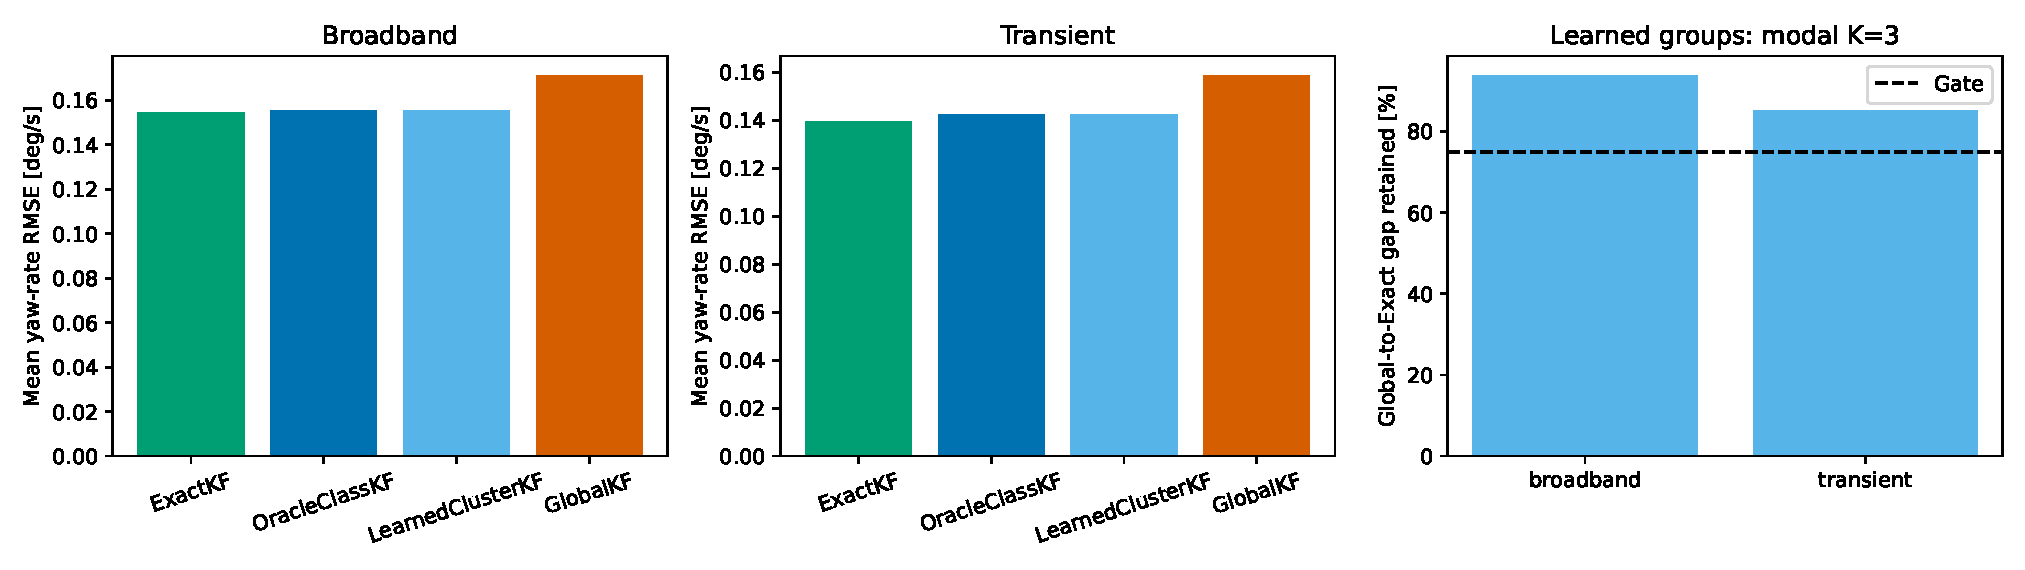
\includegraphics[width=0.98\linewidth]{../results/figures/experiment_10hc_learned_observer_groups.pdf}
\caption{Confirmation output-feedback performance and retained observer gap in
Experiment 10H-C.}
\label{fig:experiment10hc}
\end{figure}

\paragraph{Gate decision and scientific meaning.}
All predefined gates pass: modal $K=3$, positive gap-recovery intervals,
at least 75\% retained gap at every endpoint, no more than 5\% tracking excess
over OracleClassKF, and finite trajectories throughout. Unlike the earlier
LPV experiments where collaboration was mainly a model-count compromise,
10H-C exhibits a direct control benefit from label-free compatible sharing.
Its mechanism is clear: sharing completes each client's operating-point
coverage, while clustering prevents the damaging cross-class observer bias
identified in 10H-B.

The remaining step before claiming an end-to-end CFL observer is to replace
the perturbed matrix-update oracle by locally learned observer updates from
the available production-like outputs. That experiment must preserve the
unknown-$K$ discovery and closed-loop benefit under local estimation error. A
privacy or secure-aggregation study should follow only after this end-to-end
gate, because privacy noise would otherwise be applied to an optimistic update
interface.

\paragraph{Reproducibility.}
Configuration and implementation are in
\path{code/config/experiment_10hc.json} and
\path{code/experiments/experiment_10hc_learned_observer_groups.py}.
Client-level control records, candidate BIC scores, selected cardinalities,
ARI diagnostics, paired comparisons, gap-retention intervals, gate decisions,
and provenance hashes are stored under \path{results}.
